\begin{figure*}[t]
\centering
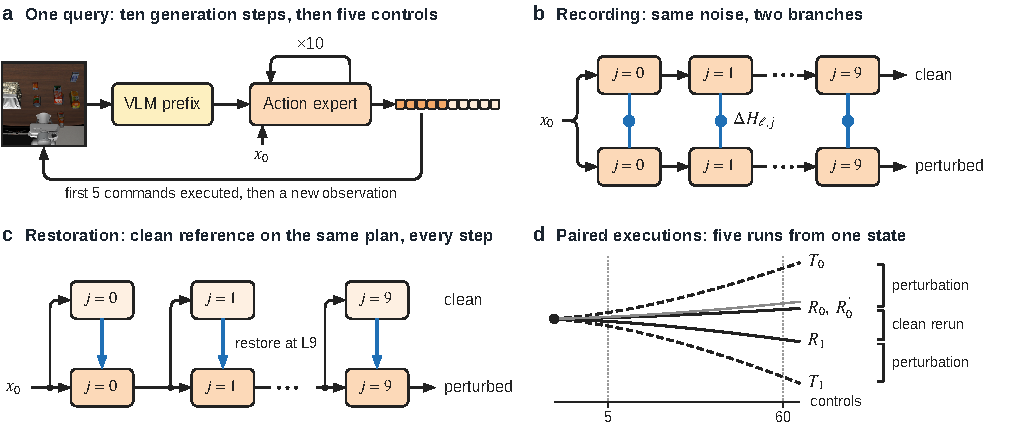
\includegraphics[width=\textwidth]{revised_figures/figure2_v3.pdf}
\caption{\textbf{How the policy runs, and what each study compares.}
(a) One query: the prefix is computed once; the action expert refines the plan from policy noise $x_0$ over ten generation steps, and the first five actions (filled) are executed before the next observation.
(b) Internal recordings: a clean and a perturbed branch start from the same $x_0$ and refine their plans separately; the response $\Delta H_{\ell,j}$ is their difference at generation step $j$ and recorded layer $\ell$.
(c) Restoration: at every generation step of every query, the policy is also run on a clean observation of the perturbed run's current state, with the same partly refined plan (top row). The clean values along the 16 shared directions are copied into the perturbed run after L9, and generation continues with the perturbed prefix.
(d) Paired executions: the distance between a perturbed run $T_i$ and the clean run $R_i$ with the same policy noise, after 5 and 60 controls, is compared with the distance between the two clean runs $R_0$ and $R_1$ (clean rerun); $R'_0$ repeats $R_0$ with the same noise. Trajectories are schematic.}
\label{fig:model-measurement}
\end{figure*}
